\documentclass[runningheads]{llncs}
\usepackage[T1]{fontenc}
\usepackage{amsmath,amssymb,booktabs,graphicx,multirow}
\usepackage{tikz}
\usetikzlibrary{arrows.meta,shapes.geometric,decorations.pathreplacing,calc,shadows}
\usepackage[hidelinks]{hyperref}
\setlength{\emergencystretch}{1.5em}
\newcommand{\Hpost}{H_{\mathrm{post}}}
\newcommand{\Hpre}{H_{\mathrm{pre}}}
\begin{document}
\title{The Oracle Gap Has a Floor: Separating Luck from Headroom in Evaluating Label Acquisition}
\titlerunning{The Oracle Gap Has a Floor}
\author{Anonymous Authors}
\authorrunning{Anonymous Authors}
\institute{Anonymous Institution}
\maketitle

\begin{abstract}
Active-learning benchmarks measure headroom with oracles that choose labels after seeing them, and read the oracle's lead as room for improvement. When outcomes are random, part of that lead is luck: some feasible label set turns out well, and only hindsight can identify it. We separate the oracle gap into evaluation-set reuse, an aleatoric floor (the value of perfect information about the acquired labels, which no strategy choosing from the same candidates can attain) and the gain of a held-out ex-ante selector. We bound the floor without distributional assumptions and estimate all three parts on real data. Across eight credit, readmission, marketing, e-mail and digit cohorts and three learners, the floor is material in nearly every cohort. Its share of the gap rises with label noise across cohorts (Spearman $0.83$) and within cohorts under injected label flips (3/3); it reaches 79\% on noisy credit outcomes but only 13--16\% on digits and spam. In 12-candidate pools, exhaustive search over all feasible sets gives the same decomposition as the greedy benchmark oracle. A risk-constrained acquisition case study shows the consequence: strategies can only compete for the part of the gap left after removing reuse and luck.
\keywords{Active learning \and Evaluation \and Oracle bounds \and Aleatoric uncertainty \and Value of information}
\end{abstract}

% ======================================================================
\section{Introduction}
\label{sec:intro}
How much better could a label-acquisition strategy be? Active-learning research increasingly answers with an \emph{oracle}: a selector that, unlike any deployable strategy, may look at the labels it acquires and at the evaluation data, and so traces the best attainable learning curve. Recent benchmarks build greedy oracles that add, step by step, the candidate whose \emph{realized} label most improves test performance~\cite{werner2023comparable,werner2024cdalbench}, and best-of-strategies oracles that pick, per batch, the strategy whose labeled batch helps most~\cite{huseljic2026boss}. The distance between oracle and practical strategies is then read as headroom; state-of-the-art strategies are reported to ``fall noticeably short of oracle performance''~\cite{huseljic2026boss}. This is part of a broader effort to make active-learning evaluation reliable~\cite{luth2023navigating,ji2023randomness}.

An oracle that selects with realized labels is an \emph{ex-post} benchmark. Part of its advantage is unreachable by construction. If an applicant's repayment, a patient's readmission or a customer's response is random given the covariates, then among all label sets a strategy could have bought, some will be lucky, and only an observer of the outcomes can pick that one. Werner et al.\ already note that their oracle overfits the test set~\cite{werner2023comparable}; outcome luck in the training labels is a second, separate source of unreachable lead, and it does not disappear when the test set is split. The distinction between ex-ante and ex-post regret is familiar in decision-focused learning~\cite{schutte2023robust}, and in bandits expected regret exceeds pseudo-regret by a noise-driven term~\cite{bubeck2012regret,audibert2010regret}. What is missing for label acquisition is a way to \emph{measure} this term on real data, and evidence of how large it is.

We make three contributions, graded by the kind of evidence behind them.
\begin{itemize}
\item \textbf{Definitions and bounds.} For a fixed family of feasible label sets we define the aleatoric floor $F$ as the expected value of perfect information about the acquired labels~\cite{howard1966information}, and prove distribution-free lower and upper bounds that hold for any dependence between sets (Section~\ref{sec:protocol}). We also show how the greedy benchmark oracle's lead splits into evaluation-set reuse, a residual and the gain of a cross-fitted ex-ante selector, and we state what this accounting does and does not identify.
\item \textbf{A measurement protocol for real data}, using an outcome model fitted on disjoint records. It recovers known-probability values on semi-synthetic data, matches recorded-outcome hindsight on real labels, and, in pools small enough to enumerate all feasible sets, gives the same decomposition under exhaustive and greedy search (Section~\ref{sec:validation}).
\item \textbf{Empirical findings} across eight cohorts and three learners (Section~\ref{sec:findings}). The floor is material in nearly every cohort, its share of the oracle gap tracks label noise both across cohorts and under within-cohort label-flip interventions, and it grows with the acquisition budget. On noisy outcomes most of what looks like headroom is reuse and luck; on near-deterministic labels most of the oracle's lead is real. A case study of risk-constrained acquisition with delayed labels, including our own conservative policy DC-PRISM, shows which strategies win the remaining gap and why that depends on the learner (Sections~\ref{sec:findings}--\ref{sec:replay}).
\end{itemize}

\begin{figure}[t]
 \centering
 \resizebox{\linewidth}{!}{% =====================================================================
% Framework figure with characters (TikZ, editable). Scaled to \linewidth by \resizebox in main.tex.
% Needs: \usepackage{tikz}
%        \usetikzlibrary{arrows.meta,shapes.geometric,decorations.pathreplacing,calc,shadows}
% Colour code used throughout the paper:
%   blue = deployable (ex-ante) part, orange = aleatoric floor, gray = test-set reuse.
% Bar proportions follow the real-label row of Table 1 (12% reuse, 52% floor, 36% deployable).
% Coordinates are in cm. Characters: \person{x}{y-feet}{scale}{shirt}{hair};
% candidates: \applicant{x}{y}{size}{risk colour}. Previous version: framework_v1_no_characters.tex
% =====================================================================
\definecolor{dep}{HTML}{4C78A8}\definecolor{flo}{HTML}{F58518}\definecolor{reu}{HTML}{9D9D9D}
\definecolor{lowr}{HTML}{54A24B}\definecolor{midr}{HTML}{EECA3B}\definecolor{highr}{HTML}{E45756}
\colorlet{shirtB}{dep!80}\colorlet{shirtC}{flo!85}\colorlet{shirtD}{teal!75}\colorlet{neutral}{black!45}
\definecolor{skin}{HTML}{F2C9A0}\definecolor{hairA}{HTML}{3B2F2F}\definecolor{hairB}{HTML}{8C5A3C}\definecolor{hairC}{HTML}{2E2E3A}
\begin{tikzpicture}[
  font=\sffamily\small, >={Stealth[length=2mm]},
  panel/.style={draw=#1!55, fill=#1!6, rounded corners=6pt, line width=0.7pt},
  ptitle/.style={font=\sffamily\normalsize\bfseries, anchor=north west, text=black!85},
  step/.style={circle, fill=#1, text=white, font=\sffamily\footnotesize\bfseries, inner sep=1.4pt},
  flow/.style={->, line width=1.1pt, draw=black!55},
  thin/.style={draw=black!45, line width=0.5pt},
  card/.style={draw=black!25, fill=white, rounded corners=3pt, drop shadow={opacity=0.15, shadow xshift=0.4pt, shadow yshift=-0.4pt}},
  bubble/.style={draw=black!35, fill=white, ellipse, inner sep=1pt, drop shadow={opacity=0.12, shadow xshift=0.3pt, shadow yshift=-0.3pt}},
]
% ---------------------------------------------------------------- characters and icons
\newcommand{\person}[5]{% x, y (feet), scale, shirt colour, hair colour
  \begin{scope}[shift={(#1,#2)}, scale=#3]
    \fill[#4] (-0.40,0) .. controls (-0.42,0.50) and (-0.26,0.70) .. (0,0.70) .. controls (0.26,0.70) and (0.42,0.50) .. (0.40,0) -- cycle;
    \fill[#4!70!black] (-0.06,0.70) -- (0,0.55) -- (0.06,0.70) -- cycle;
    \fill[skin] (-0.07,0.66) rectangle (0.07,0.78);
    \fill[skin] (0,0.98) circle (0.24);
    \fill[#5] (-0.25,1.00) .. controls (-0.25,1.30) and (0.25,1.30) .. (0.25,1.00)
              .. controls (0.12,1.10) and (-0.12,1.12) .. (-0.25,1.00) -- cycle;
    \fill[black!80] (-0.08,0.97) circle (0.025); \fill[black!80] (0.08,0.97) circle (0.025);
    \draw[black!60, line width=0.35pt] (-0.06,0.88) .. controls (-0.02,0.85) and (0.02,0.85) .. (0.06,0.88);
  \end{scope}}
\newcommand{\applicant}[4]{% x, y, size r, colour : small person icon (applicant)
  \fill[#4, opacity=0.9] ($(#1,#2)+(-#3,-1.05*#3)$) arc (180:0:#3 and 0.85*#3) -- cycle;
  \fill[#4!80!black] ($(#1,#2)+(0,0.25*#3)$) circle (0.52*#3);}
\newcommand{\die}[3]{% x, y, size
  \draw[card] (#1,#2) rectangle ++(#3,#3);
  \foreach \dx/\dy in {0.25/0.25,0.75/0.25,0.5/0.5,0.25/0.75,0.75/0.75}
    \fill[black!70] ($(#1,#2)+(\dx*#3,\dy*#3)$) circle (0.045*#3/0.35);}
\newcommand{\padlock}[3]{% x, y, size
  \draw[white, line width=1.3pt] ($(#1,#2)+(-0.26*#3,0.28*#3)$) -- ++(0,0.22*#3) arc (180:0:0.26*#3) -- ++(0,-0.22*#3);
  \fill[white, rounded corners=1pt] ($(#1,#2)+(-0.42*#3,-0.30*#3)$) rectangle ($(#1,#2)+(0.42*#3,0.30*#3)$);
  \fill[flo] ($(#1,#2)+(0,0.04*#3)$) circle (0.08*#3);}

% ================================================================ PANEL 1: acquisition
\draw[panel=gray] (0,0) rectangle (4.2,5.6);
\node[step=black!70] at (0.32,5.28) {1};
\node[ptitle] at (0.55,5.48) {Acquire under risk};
\foreach \x/\y/\r/\c in {1.55/4.45/0.13/lowr, 2.05/4.65/0.15/lowr, 2.55/4.40/0.11/lowr, 3.05/4.70/0.18/midr, 3.60/4.35/0.20/highr,
                         1.70/3.80/0.17/midr, 2.25/3.95/0.12/lowr, 2.80/3.75/0.13/lowr, 3.35/3.85/0.22/highr,
                         1.60/3.10/0.12/lowr, 2.15/3.20/0.19/highr, 2.70/3.05/0.13/midr, 3.25/3.15/0.12/lowr, 3.75/3.30/0.16/midr}
  {\applicant{\x}{\y}{\r}{\c}}
\draw[dashed, line width=0.9pt, draw=dep, rounded corners=8pt] (1.25,4.05) -- (1.28,4.95) -- (2.85,5.00) -- (3.05,4.18) -- (3.05,3.50) -- (2.45,3.40) -- (1.32,3.48) -- cycle;
\node[font=\sffamily\footnotesize, text=dep, anchor=west] at (1.10,2.62) {feasible: $R_\alpha(S)\le B$};
\person{0.62}{0.95}{1.05}{dep}{hairA}
\draw[card] (0.98,1.25) rectangle (1.32,1.70); \foreach \yy in {1.36,1.46,1.56} {\draw[black!40] (1.04,\yy) -- (1.26,\yy);}
\node[font=\sffamily\footnotesize, text=black!70, align=left, anchor=west] at (1.45,1.62) {lender buys labels\\ by approving};
\applicant{1.25}{0.66}{0.09}{lowr}\applicant{1.50}{0.66}{0.09}{midr}\applicant{1.75}{0.66}{0.09}{highr}
\node[anchor=west, font=\sffamily\footnotesize, text=black!65] at (1.86,0.66) {risk};
\applicant{2.62}{0.66}{0.07}{neutral}\applicant{2.88}{0.66}{0.13}{neutral}
\node[anchor=west, font=\sffamily\footnotesize, text=black!65] at (3.02,0.66) {size};
\node[font=\sffamily\footnotesize, text=black!55] at (2.10,0.24) {history $+$ pending $+$ pool};

% ================================================================ PANEL 2: two oracles
\draw[panel=violet] (4.65,0) rectangle (9.75,5.6);
\node[step=black!70] at (4.97,5.28) {2};
\node[ptitle] at (5.20,5.48) {Two oracles};
\person{5.45}{3.05}{0.95}{shirtB}{hairB}
\node[anchor=west, font=\sffamily\small\bfseries, text=dep] at (5.00,2.72) {ex-ante};
\node[bubble, minimum width=3.15cm, minimum height=1.55cm] (tb) at (7.75,3.95) {};
\fill[white, draw=black!35] (6.20,3.55) circle (0.07); \fill[white, draw=black!35] (6.02,3.40) circle (0.045);
\die{6.65}{3.70}{0.30}\die{6.95}{3.95}{0.30}\die{6.95}{3.47}{0.30}
\draw[->, black!55, line width=0.8pt] (7.35,3.88) -- (7.62,3.88);
\foreach \i/\h in {0/0.62,1/0.38,2/0.52,3/0.70} {\fill[dep!75] (7.75+\i*0.27,3.45) rectangle ++(0.18,\h);}
\draw[line width=1pt, dep] (7.98,3.38) -- (8.20,3.38);
\node[font=\sffamily\footnotesize, text=black!70, align=left, anchor=west] at (6.45,2.68) {best by \emph{expected} loss\\ over label replicates};
\draw[violet!30, line width=0.6pt] (4.85,2.32) -- (9.55,2.32);
\person{5.45}{0.45}{0.95}{shirtC}{hairC}
\node[anchor=west, font=\sffamily\small\bfseries, text=flo] at (5.00,0.18) {ex-post};
\fill[flo!35] (6.55,0.40) -- (7.25,0.40) -- (7.10,0.62) -- (6.70,0.62) -- cycle;
\shade[inner color=white, outer color=violet!40] (6.90,1.15) circle (0.50); \draw[violet!60] (6.90,1.15) circle (0.50);
\node[text=lowr!80!black, font=\small] at (6.75,1.25) {$\checkmark$};
\node[text=highr, font=\small] at (7.05,1.02) {$\times$};
\draw[flo, line width=0.8pt, dashed, ->] (5.95,1.45) .. controls (6.15,1.70) and (6.30,1.65) .. (6.42,1.45);
\node[font=\sffamily\footnotesize, text=black!70, align=left, anchor=west] at (7.50,1.20) {best after\\ seeing the\\ \emph{realized} labels};

% ================================================================ PANEL 3: decomposition
\draw[panel=orange] (10.20,0) rectangle (13.50,5.6);
\node[step=black!70] at (10.52,5.28) {3};
\node[ptitle] at (10.75,5.48) {Split the gap};
\def\bx{10.50}\def\bw{0.62}
\fill[reu] (\bx,0.55) rectangle ++(\bw,0.50);
\fill[flo] (\bx,1.05) rectangle ++(\bw,2.15);
\fill[dep] (\bx,3.20) rectangle ++(\bw,1.48);
\draw[white, line width=1pt] (\bx,1.05) -- ++(\bw,0) (\bx,3.20) -- ++(\bw,0);
\padlock{\bx+0.31}{2.12}{0.46}
\node[font=\sffamily\scriptsize\bfseries, text=black!75] at (\bx+0.31,4.84) {reported};
\draw[decorate, decoration={brace, amplitude=4pt}, thin] (\bx+\bw+0.08,4.66) -- (\bx+\bw+0.08,3.22);
\draw[decorate, decoration={brace, amplitude=4pt}, thin] (\bx+\bw+0.08,3.18) -- (\bx+\bw+0.08,1.07);
\draw[decorate, decoration={brace, amplitude=3pt}, thin] (\bx+\bw+0.08,1.03) -- (\bx+\bw+0.08,0.57);
\node[anchor=west, align=left, font=\sffamily\footnotesize] at (\bx+\bw+0.25,3.94) {\textbf{\textcolor{dep}{deployable}}\\ \textbf{\textcolor{dep}{gap}}\\ (gainable)};
\node[anchor=west, align=left, font=\sffamily\footnotesize] at (\bx+\bw+0.25,2.12) {\textbf{\textcolor{flo}{aleatoric}}\\ \textbf{\textcolor{flo}{floor}}\\ (luck in\\ the labels)};
\node[anchor=west, align=left, font=\sffamily\footnotesize] at (\bx+\bw+0.25,0.80) {\textbf{\textcolor{black!60}{test reuse}}};

% ================================================================ PANEL 4: predict and act
\draw[panel=teal] (13.95,0) rectangle (18.10,5.6);
\node[step=black!70] at (14.27,5.28) {4};
\node[ptitle] at (14.50,5.48) {Audit and act};
\draw[->, thin] (15.35,3.05) -- (17.80,3.05) node[above left, font=\sffamily\footnotesize, text=black!65, xshift=2pt, yshift=1pt] {noise};
\draw[->, thin] (15.35,3.05) -- (15.35,4.85) node[right, font=\sffamily\footnotesize, text=black!65, xshift=1pt, yshift=-4pt] {floor share};
\draw[flo, line width=1.2pt] plot[smooth, tension=0.6] coordinates {(15.50,3.25) (16.05,3.40) (16.60,3.85) (17.15,4.30) (17.60,4.55)};
\foreach \x/\y in {15.60/3.22,16.10/3.48,16.50/3.75,16.85/4.15,17.20/4.25,17.50/4.60} {\fill[flo!80!black] (\x,\y) circle (0.05);}
\person{14.55}{2.95}{0.85}{shirtD}{hairB}
\draw[black!70, line width=1.4pt] (14.92,3.72) -- (15.06,3.88);
\draw[black!70, line width=1pt, fill=white, fill opacity=0.6] (15.18,4.02) circle (0.18);
\node[font=\footnotesize, text=black!80, align=center] at (16.10,2.20) {$F_{\mathrm{lo}}\le F\le F_{\mathrm{up}}$\\[1pt]
  \scriptsize distribution-free floor bounds};
\begin{scope}[shift={(16.05,1.12)}]
  \fill[dep!25, opacity=0.9] (-0.50,0) circle (0.62); \fill[lowr!30, opacity=0.9] (0.50,0) circle (0.62);
  \draw[dep, line width=0.8pt] (-0.50,0) circle (0.62); \draw[lowr!80!black, line width=0.8pt] (0.50,0) circle (0.62);
  \node[font=\sffamily\footnotesize, text=dep!80!black] at (-0.60,0) {proxy};
  \node[font=\sffamily\footnotesize, text=lowr!50!black] at (0.58,0) {learner};
\end{scope}
\node[font=\sffamily\footnotesize, text=black!70] at (16.05,0.28) {match $\Rightarrow$ gap closed};

% ================================================================ flows between panels
\draw[flow] (4.20,2.80) -- (4.65,2.80);
\draw[flow, draw=dep]  (9.75,3.95) -- (10.20,3.95);
\draw[flow, draw=flo]  (9.75,1.20) -- (10.20,1.20);
\draw[flow] (13.50,2.80) -- (13.95,2.80);

% ================================================================ bottom strip: estimation on real data
\draw[panel=gray] (0,-1.75) rectangle (18.10,-0.40);
\node[font=\sffamily\small\bfseries, anchor=west, text=black!80] at (0.20,-1.07) {Estimation on real data};
\node[cylinder, shape border rotate=90, aspect=0.25, draw=black!55, fill=white, minimum height=0.85cm, minimum width=0.62cm] (db) at (4.45,-1.07) {};
\foreach \yy in {-1.25,-1.08,-0.91} {\draw[black!30] (4.17,\yy) -- (4.73,\yy);}
\node[anchor=west, font=\sffamily\footnotesize, align=left] at (4.80,-1.07) {disjoint\\ records};
\draw[flow] (6.05,-1.07) -- (6.40,-1.07);
\node[card, font=\sffamily\footnotesize, inner sep=3pt] at (7.35,-1.07) {$\hat p$ (boosting)};
\draw[flow] (8.32,-1.07) -- (8.62,-1.07);
\die{8.72}{-1.27}{0.38}\die{9.18}{-1.27}{0.38}
\node[anchor=west, font=\sffamily\footnotesize, align=left] at (9.70,-1.07) {label replicates $Y^{(r)}$\\ feed both oracles};
\node[anchor=west, font=\sffamily\footnotesize, text=lowr!70!black] at (13.55,-0.85) {$\checkmark$ recovers known-$p$ values};
\node[anchor=west, font=\sffamily\footnotesize, text=lowr!70!black] at (13.55,-1.30) {$\checkmark$ greedy $\approx$ exact search};
\draw[->, dashed, draw=black!45, line width=0.8pt] (7.35,-0.40) -- (7.35,-0.05);
\end{tikzpicture}
}
 \caption{Overview. (1) A lender buys labels by approving applicants, under a risk budget. (2) The ex-ante oracle picks the set with the best \emph{expected} loss over outcome replicates; the ex-post oracle picks after seeing the \emph{realized} labels. (3) The reported oracle gap splits into test reuse, the aleatoric floor and a deployable part. (4) Bounds and noise diagnostics audit the floor; whether a strategy closes the deployable part depends on whether its information proxy matches the learner. Bottom: an outcome model $\hat p$ fitted on disjoint records generates label replicates for both oracles.}
 \label{fig:framework}
\end{figure}

% ======================================================================
\section{Setting}
\label{sec:setting}
At round $t$ a learner holds a labeled history $D_t$, the covariates of pending acquisitions $O_t$ (selected but not yet resolved), an unlabeled candidate pool $C_t$ and target covariates $Q_t$. Candidate $i$ has a binary outcome $Y_i$, revealed only after acquisition, and a visible exposure $e_i\ge0$. A strategy chooses $S_t\subseteq C_t$ from the visible information $\mathcal H_t$. Learning is measured by the Brier score~\cite{brier1950verification} of a downstream learner (an $\ell_2$-logistic model, gradient boosting or a one-hidden-layer network); $L(S;Y)$ is its test loss after fitting on $D\cup O\cup S$, where $Y$ collects the hidden training outcomes of $O$ and $S$.

\paragraph{Risk budget.} In our main application, acquiring a label is an action with exposure: a lender observes repayment only by approving an applicant~\cite{lakkaraju2017selective,wei2021selective}, and labels of earlier approvals are still pending. With a risk score $q_i$, $\ell=\log(1/\alpha)$ and $\phi(q)=q(1-q)$ for $q\le\frac12$ ($\frac14$ otherwise), a set is feasible if
\begin{equation}
 R_\alpha(S)=\sum_{i\in S}e_iq_i+\Big(2\ell\sum_{i\in S}e_i^2\phi(q_i)\Big)^{1/2}+\frac{\ell}{3}\max_{i\in S}e_i\le B_t .
 \label{eq:envelope}
\end{equation}
This is a sub-gamma tail bound~\cite{boucheron2013concentration}: if outcomes are conditionally independent and $p_i\le q_i$, realized adverse exposure exceeds $R_\alpha(S)$ with probability at most $\alpha=0.1$. Our scores (a Wilson-shifted~\cite{wilson1927probable} upper quantile of 40 Laplace draws of the fitted logit) do not guarantee $p_i\le q_i$, so we treat~\eqref{eq:envelope} as an \emph{operational} risk budget shared by all strategies. $B_t$ is $1.03$ times the envelope of the $k$ lowest-risk candidates ($k=6$ unless stated). The \emph{quantity reference} $M_K$ is the largest feasible set; we find it by enumeration for up to 16 candidates and otherwise by an exposure-stratified search, whose cardinality was certified in 1{,}320 of 1{,}408 states and confirmed by exact branch-and-bound in the remaining 88. For cohorts without a natural exposure we set $e_i=1$, so the budget is a cardinality-like constraint.

% ======================================================================
\section{Decomposing the Oracle Gap}
\label{sec:protocol}
\paragraph{Family oracles and the floor.} Fix the visible information $\mathcal H$ and a finite family $\mathcal F$ of feasible sets, constructed from $\mathcal H$ only and containing $M=M_K$. Let $\bar L(S;Y)$ be the test loss with test-label noise integrated out, and write the gain of $S$ over the quantity reference as $d_S=\bar L(M;Y)-\bar L(S;Y)$, with mean $\mu_S=\mathbb E[d_S\mid\mathcal H]$. Two oracles are natural:
\begin{equation}
 \Hpost=\mathbb E\big[\max_{S\in\mathcal F}d_S\mid\mathcal H\big],\qquad
 \Hpre=\max_{S\in\mathcal F}\mu_S .
\end{equation}
$\Hpost$ is the lead of an oracle that chooses after seeing the hidden training labels; $\Hpre$ is the lead of the best choice that does not see them. Their difference
\begin{equation}
 F=\Hpost-\Hpre\ \ge 0
\end{equation}
is the \emph{aleatoric floor}. It is the expected value of perfect information about the training outcomes~\cite{howard1966information,raiffa1961applied}: no strategy that chooses from $\mathcal F$ on the basis of $\mathcal H$ can attain it, since such a strategy's expected gain $\Gamma_\pi$ is at most $\Hpre$. Hence
\begin{equation}
 \Hpost-\Gamma_\pi = F+(\Hpre-\Gamma_\pi),
\end{equation}
and only the second term, the \emph{selection gap}, is open to better strategies. Two qualifications matter. First, $F$ is defined relative to $\mathcal F$ and $\mathcal H$: a strategy with more information, or a larger candidate family, faces a different floor. Second, $F$ is not a property of the labels alone; it depends on how strongly the learner's test loss responds to which labels it receives.

\paragraph{Distribution-free bounds.} Let $b$ maximize $\mu_S$ and let $r\in\mathcal F$ be any other set.
\begin{proposition}\label{prop:bounds}
For any joint distribution of $(d_S)_{S\in\mathcal F}$ with finite means,
\begin{equation}
 F_{\mathrm{lo}}:=\mathbb E(d_r-d_b)_+\ \le\ F\ \le\ \mathbb E\max_{S\in\mathcal F}(d_S-\mu_S)=:F_{\mathrm{up}} .\label{eq:bounds}
\end{equation}
The same inequalities hold exactly when expectations are replaced by averages over any finite set of outcome replicates, including when $b$ and $r$ are chosen from those replicates.
\end{proposition}
\begin{proof}
Pointwise, $\max_S d_S\ge\max(d_b,d_r)=d_b+(d_r-d_b)_+$; taking expectations and subtracting $\mu_b=\Hpre$ gives the lower bound. Also $\max_S d_S\le\max_S\mu_S+\max_S(d_S-\mu_S)$ pointwise, which gives the upper bound. Both arguments use only linearity and monotonicity of the average, so they apply to the empirical distribution. \qed
\end{proof}
The lower bound says that the floor is at least the expected regret of committing to the best set when its closest competitor $r$ sometimes does better; it is large when leading sets are nearly tied and their outcomes disagree. If the centered gains are jointly Gaussian with standard deviations $\sigma_S$, then $F\le\max_S\sigma_S\sqrt{2\log|\mathcal F|}$ under any correlation structure, and if $d_b-d_r$ is normal with mean $\Delta$ and standard deviation $s$, then $F_{\mathrm{lo}}=s\varphi(\Delta/s)-\Delta\Phi(-\Delta/s)$. These closed forms rely on the Gaussian assumption; Proposition~\ref{prop:bounds} does not. The empirical inequalities provide no confidence statement about population $F$, so we report sampling uncertainty separately.

\paragraph{What the benchmark oracle measures.} Benchmarks select a batch greedily using realized labels and an evaluation set~\cite{werner2023comparable,werner2024cdalbench}. We split the test records into halves $T_1,T_2$ and generate $R$ replicates of the hidden training outcomes. Let $G_{\mathrm{rep}}$ be the mean gain over $M$ of the greedy oracle that selects and is scored on $T_1$ (the \emph{reported} gap), $G_{\mathrm{hold}}$ the gain of the same selections scored on $T_2$, and $G_{\mathrm{cf}}$ the gain of a greedy selector that chooses by mean $T_1$ loss over one half of the replicates and is scored on $T_2$ over the other half, with halves exchanged and averaged. Then
\begin{equation}
 G_{\mathrm{rep}}=\underbrace{(G_{\mathrm{rep}}-G_{\mathrm{hold}})}_{\text{test reuse}}+\underbrace{(G_{\mathrm{hold}}-G_{\mathrm{cf}})}_{\text{residual}}+\underbrace{G_{\mathrm{cf}}}_{\text{cross-fitted gain}} .\label{eq:greedy}
\end{equation}
This is an accounting identity. The residual is the benchmark counterpart of the floor: the extra gain from choosing with the realized rather than the expected outcomes. It coincides with $F$ only if both selectors search the same space without error and the replicate banks are large. Search error and finite banks both enter the residual, in opposite directions: plug-in maximization of estimated means overstates $\Hpre$, while cross-fitting understates it~\cite{smith2006optimizer,cawley2010overfitting}. We therefore check the identity against exhaustive search (Section~\ref{sec:validation}) and report $G_{\mathrm{cf}}$ as the gain of a specific held-out selector, not as the best deployable value.

\paragraph{Estimation on real data.} With a known outcome probability $p$, replicates are drawn from $p$ with common random numbers across sets. On real cohorts, a gradient-boosting model $\hat p$ fitted on records disjoint from every state supplies the replicates, and the recorded test labels are held fixed. The quantities above are therefore conditional on the test set and on $\hat p$. We test $\hat p$ in three ways: on semi-synthetic data where the truth is known, against the hindsight gap realized with recorded labels, and under deliberate perturbations of $\hat p$.

% ======================================================================
\section{Strategies and Studies}
\label{sec:policy}
\paragraph{Strategies.} All strategies share the state, the scores $q$, the budget and~\eqref{eq:envelope}. \emph{Safe-MinRisk} returns $M_K$; \emph{fixed count} takes a fixed fraction of $K=|M_K|$ by point value; \emph{Fisher-cost} packs by single-label variance reduction per unit exposure. Four rules pack greedily until no feasible candidate remains: \emph{Random}, \emph{Uncertainty}~\cite{lewis1994sequential}, \emph{BAIT-greedy} on $\operatorname{tr}(F_Q(H_{D+O}+A_S)^{-1})$~\cite{ash2021fishing} and \emph{TargetVar-greedy} on the target-weighted proxy
\begin{equation}
 V_\theta(S)=\operatorname{tr}\big[W_Q\{H_{D+O}^{-1}-(H_{D+O}+A_S)^{-1}\}\big],\label{eq:value}
\end{equation}
where $H_{D+O}$ is the logistic Fisher information of history and pending covariates, $A_S$ that of $S$, and $W_Q$ weights target directions by their Brier sensitivity~\cite{yu2006transductive,bickfordsmith2023prediction}. \emph{Proxy-argmax} takes $\arg\max V_{\hat\theta}$ over the evaluation family. \emph{DC-PRISM}, the conservative policy we designed for this setting, evaluates~\eqref{eq:value} on a family anchored at $M_K$ under 20 Laplace parameter draws~\cite{mackay1992practical}, scores each set by the 0.2-quantile of $\tanh\{(V_m(S)-V_m(M_K))/2.5V_m(M_K)\}$ minus a quantity penalty $0.22(K-|S|)_+/K$, and returns $M_K$ unless the best score exceeds $0.08$ (about 50\,ms per decision with 24 candidates). All information proxies come from the logistic model.

\paragraph{Families.} The family $\mathcal F$ contains $M_K$, the choices of all strategies above and sets built from visible information around them (22--27 sets per state). Adding 64 random feasible sets (81--88 sets) leaves the estimated deployable share $\Hpre/\Hpost$ essentially unchanged: 80--83\% in controlled worlds at every sub-family size from 2 to 80, and 6--38\% on semi-synthetic states, where it rises slightly with $|\mathcal F|$. The deployable share is thus not an artifact of a small family.

\paragraph{Cohorts and states.} We use four credit cohorts (HMEQ~\cite{sasHMEQ}, LendingClub~\cite{lendingclubSource}, PPDai~\cite{ppdaiSource,he2018ensemble} and UCI Credit~\cite{yeh2009comparison}), 30-day hospital readmission~\cite{strack2014impact} with days in hospital as exposure, bank-marketing subscription~\cite{moro2014bank}, Spambase~\cite{hopkins1999spambase} and USPS digits~\cite{hull1994usps} ($\ge5$ versus $<5$), the last both as raw pixels and as 10 principal components. Each state is the first round of a delayed replay with 68 historical labels, 14 pending and 24 candidate records. Candidates are drawn at random (the \emph{natural} stream) or, for credit and readmission, also from an \emph{engineered} stream that mixes low-risk, pending-aligned, complementary and tail candidates. Controlled worlds and \emph{semi-synthetic} states (real covariates, outcomes from a known logit) provide known~$p$.

\paragraph{Statistics.} Every study fixed its states, seeds, families, predictions and a material-effect threshold of $0.5\times10^{-3}$ Brier before running, with protocol and code frozen in version control. We report paired means with 95\% Bonferroni simultaneous intervals and Holm-adjusted tests~\cite{holm1979simple}, and use two one-sided tests at the material margin when we claim agreement. All values are in units of $10^{-3}$ Brier.

% ======================================================================
\section{Validating the Protocol}
\label{sec:validation}
\paragraph{Known probabilities are recovered.} On 512 semi-synthetic states, boosting $\hat p$ fitted on auxiliary records labeled from the true $p$ gives estimates whose bias relative to the known-$p$ protocol lies within $\pm0.5$ in 95 of 96 checks (8 groups $\times$ 12 quantities). Mean biases of $\Hpost$, $\Hpre$, the floor and the main strategy gains are at most $0.20$, and state-level correlations for $\Hpre$ are $0.73$--$0.95$. A logistic $\hat p$ underestimates $\Hpre$ by $0.26$--$0.28$ when the true logit is nonlinear, so the protocol requires a flexible outcome model.

\paragraph{Recorded outcomes agree with simulated hindsight.} With real labels, the hindsight gap can also be computed once on the recorded training outcomes and compared with its $\hat p$-simulated expectation. For the logistic and boosting learners the point estimates agree within $0.54$ in all 20 cohort--stream--learner cells, and in 11 of them the 95\% interval of the difference lies inside $\pm0.5$. In 192 further states across eight cohorts, the pooled difference in the reported greedy gap has 90\% interval $[-0.09,0.42]$, which establishes equivalence at the $0.5$ margin; for the held-out greedy gap the interval $[-0.14,0.51]$ narrowly misses it. With the neural learner, eight of nine cohorts agree but PPDai does not (simulated $7.39$ versus realized $5.01$), so we treat neural-learner floors on PPDai with caution.

\paragraph{The floor moves with the sharpness of $\hat p$, as it should.} On 64 known-$p$ states, the floor estimated with $\hat p$ has bias $-0.04$ (RMSE $0.5$). Shifting all logits by $\pm0.5$ changes the bias by at most $0.3$. Rescaling the logits changes it more: sharper probabilities (temperature $0.5$) lower the estimated floor by $0.8$, flatter ones (temperature $2$) raise it by $0.5$. This is the direction the noise mechanism predicts, and it identifies the main threat to the estimates: a miscalibrated spread of $\hat p$, which disjoint fitting and held-out calibration (ECE $0.011$--$0.027$, calibration slope $0.64$--$1.24$) reduce but cannot rule out.

\paragraph{Greedy search does not distort the decomposition.} In pools of 12 candidates every feasible set can be enumerated (on average 728 sets per state). On 192 such states over eight cohorts we computed~\eqref{eq:greedy} twice, once with greedy and once with exact search over the whole feasible space. The two agree to within $0.1$ in every cohort for reuse, residual and cross-fitted gain (pooled residual difference $-0.02$, cross-fitted gain difference $0.01$; Fig.~\ref{fig:predict}c). At this scale, therefore, neither search error nor a restricted family drives the residual. Even with exact search, the residual accounts for 47\% of the reported gap, ranging from 21\% (USPS) and 27\% (Spambase) to 76\% (PPDai, UCI Credit). We do not have an exact check for larger pools.

\paragraph{Bounds.} The empirical inequalities~\eqref{eq:bounds} hold in all 624 states of the revision study, as Proposition~\ref{prop:bounds} requires; this verifies the implementation. In stress tests with antithetic, equicorrelated, skewed and heavy-tailed gains, an upper value computed as if the gains were independent normal fails to bound $F$ in as many as all replications of a configuration, whereas~\eqref{eq:bounds} holds throughout. We therefore use only the distribution-free bounds.

% ======================================================================
\section{Findings}
\label{sec:findings}
\paragraph{Most of the benchmark gap is reuse and luck when outcomes are noisy.} Table~\ref{tab:known} applies~\eqref{eq:greedy} to five settings. In controlled worlds built to contain directional information, the cross-fitted selector keeps most of the reported gap ($21.5$ of $29.5$). On semi-synthetic states with known $p$, the reported lead of $6.9$ over the best fixed strategy disappears once reuse and the residual are removed. On real credit and readmission labels, the lead shrinks by 70--85\%. A benchmark that reports the uncorrected gap counts this part as headroom.

\begin{table}[t]
\caption{The benchmark greedy oracle under the risk budget, logistic learner ($\times10^{-3}$ Brier). Reported gap $=$ test reuse $+$ residual $+$ cross-fitted (CF) gain, Eq.~\eqref{eq:greedy}. Last column: lead over the best fixed practical strategy, reported $\to$ cross-fitted.}
\label{tab:known}
\centering\scriptsize
\setlength{\tabcolsep}{3.5pt}
\begin{tabular}{lrrrrrr}
\toprule
Setting & States & Reported & Reuse & Residual & CF gain & Lead over best \\
\midrule
Controlled worlds & 64 & 29.5 & 4.5 & 3.5 & 21.5 & 15.8$\to$7.8 \\
Semi-synthetic (known $p$) & 256 & 7.2 & 2.9 & 3.9 & 0.3 & 6.9$\to$0.0 \\
Credit, engineered stream & 128 & 8.0 & 0.6 & 4.1 & 3.3 & 6.7$\to$2.0 \\
Credit, natural stream & 128 & 3.4 & 0.8 & 1.7 & 0.9 & 3.2$\to$0.6 \\
Readmission, both streams & 64 & 2.3 & 0.3 & 1.4 & 0.5 & 2.0$\to$0.3 \\
\bottomrule
\end{tabular}
\end{table}

\paragraph{The floor's share tracks label noise.} Before running the eight-cohort study we registered the prediction that the residual share would increase with the label-noise index $\overline{\hat p(1-\hat p)}$. It does (Table~\ref{tab:gradient}, Fig.~\ref{fig:predict}a): Spearman $0.83$ ($p=0.01$) with the logistic learner and $0.67$ ($p=0.05$) with the neural learner. On Spambase and USPS, which have nearly deterministic labels, the residual takes 13--16\% of the logistic gap and the oracle's lead is mostly real; on UCI Credit and LendingClub it takes 67--79\% and the cross-fitted lead falls to $0.4$. On USPS raw pixels, the representation used in a recent benchmark~\cite{werner2024cdalbench}, the neural oracle's lead halves from $15.9$ to $8.0$, and most of the drop is reuse. The neural learner raises the reported gap on every cohort and lowers the residual share on noisy cohorts, consistent with a more flexible learner extracting more deployable information.

\begin{table}[t]
\caption{The benchmark oracle along a label-noise gradient (natural stream; 48 states per cohort for the logistic and 32 for the neural learner; $\times10^{-3}$ Brier). Noise: mean $\hat p(1-\hat p)$. Reuse and residual: \% of the reported gap. Lead: over the best fixed strategy, reported $\to$ cross-fitted.}
\label{tab:gradient}
\centering\scriptsize
\setlength{\tabcolsep}{2.6pt}
\begin{tabular}{lrrrrrrrrr}
\toprule
& & \multicolumn{4}{c}{Logistic learner} & \multicolumn{4}{c}{Neural learner (MLP)} \\
\cmidrule(lr){3-6}\cmidrule(lr){7-10}
Cohort & Noise & Gap & Reuse & Resid. & Lead & Gap & Reuse & Resid. & Lead \\
\midrule
USPS, raw pixels & 0.036 & \multicolumn{4}{c}{(neural only)} & 18.7 & 32 & 10 & 15.9$\to$8.0 \\
Spambase & 0.054 & 7.5 & 32 & 16 & 5.1$\to$1.5 & 14.1 & 25 & 29 & 11.4$\to$3.8 \\
USPS, 10 PCs & 0.065 & 10.8 & 12 & 13 & 7.7$\to$5.0 & 16.6 & 23 & 29 & 15.0$\to$6.4 \\
Readmission & 0.081 & 1.3 & 29 & 66 & 1.1$\to$$-$0.1 & 4.8 & 23 & 54 & 4.0$\to$0.3 \\
Bank Marketing & 0.091 & 4.5 & 15 & 39 & 4.1$\to$1.7 & 11.9 & 34 & 29 & 10.3$\to$2.8 \\
HMEQ & 0.101 & 3.4 & 15 & 42 & 3.0$\to$1.0 & 7.8 & 26 & 39 & 7.2$\to$2.1 \\
PPDai & 0.108 & 2.8 & 17 & 60 & 2.7$\to$0.5 & 10.4 & 20 & 38 & 9.1$\to$3.0 \\
UCI Credit & 0.136 & 3.4 & 15 & 67 & 3.2$\to$0.4 & 8.2 & 47 & 38 & 7.8$\to$0.8 \\
LendingClub & 0.144 & 2.7 & 8 & 79 & 2.8$\to$0.4 & 8.5 & 39 & 53 & 8.6$\to$0.7 \\
\bottomrule
\end{tabular}
\end{table}

\paragraph{Injecting noise raises the floor within a cohort.} A cross-cohort correlation could reflect other differences between cohorts. In a separately registered intervention we flipped training labels with probability $0$, $0.1$, $0.2$ and $0.3$ within HMEQ, Bank Marketing and USPS (16 states per dose and cohort). The family floor rises monotonically in all three cohorts (HMEQ $1.0\to2.3$, Bank Marketing $1.2\to2.9$, USPS $1.2\to3.6$), and so does the residual share (Fig.~\ref{fig:predict}b). On USPS the cross-fitted gain falls from $7.8$ to $2.9$ as the labels become noisier: the oracle's lead hardly changes, but its composition does. This supports a causal reading for randomized label corruption; natural outcome noise may differ from random flips.

\begin{figure}[t]
 \centering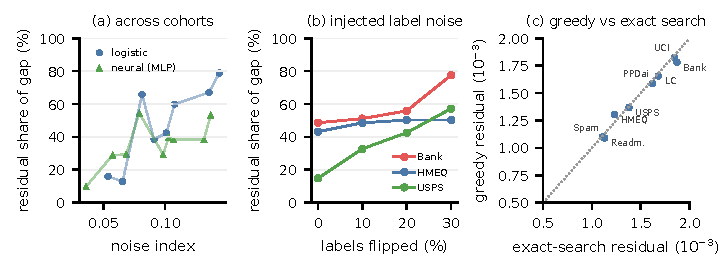
\includegraphics[width=\linewidth]{figures/fig_predict.pdf}
 \caption{(a) Residual share of the benchmark oracle gap against the label-noise index, one point per cohort (Table~\ref{tab:gradient}). (b) The same share when training labels are flipped at random within a cohort; 16 states per dose. (c) Residual under greedy search against exact search over all feasible sets, 12-candidate pools, 24 states per cohort; dotted: identity.}
 \label{fig:predict}
\end{figure}

\paragraph{Larger budgets raise the floor; larger pools need not.} Varying the budget target from 3 to 6 to 12 low-risk labels raised the measured family floor monotonically in all eight cohorts (mean $0.67\to1.06\to1.41$; paired increase from $k=3$ to $12$: $0.74$ $[0.67,0.82]$; Fig.~\ref{fig:budget}), while the deployable part moved much less uniformly. More acquired labels, rather than riskier labels, drive the increase: per-label outcome variance of the chosen sets barely changes. This is an empirical regularity, not a theorem, since $\Hpost$ and $\Hpre$ both change with the budget. Enlarging the candidate pool from 24 to 48 to 96 at a fixed budget produced no consistent pattern (the floor rose on HMEQ, rose and fell on Bank Marketing and USPS), so we make no claim about pool size.

\begin{figure}[t]
 \centering
 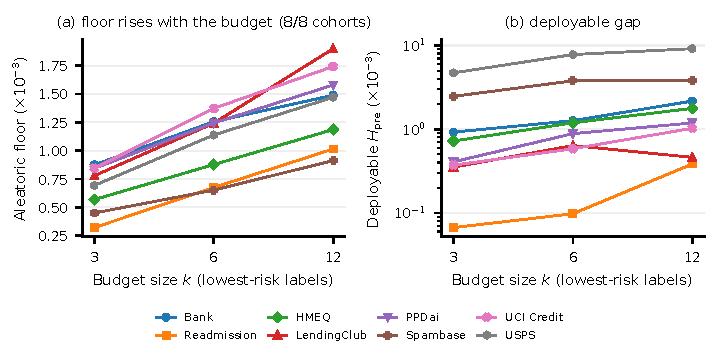
\includegraphics[width=\linewidth]{figures/fig_budget.pdf}
 \caption{The risk budget as a lever (logistic learner, 32 states per cohort and budget; the budget is sized for the $k$ lowest-risk candidates). (a) The family floor rises with $k$ in all eight cohorts. (b) The deployable part $\Hpre$ (cross-fitted, log scale) moves much less uniformly.}
 \label{fig:budget}
\end{figure}

\paragraph{Who closes the deployable part depends on the learner.} Table~\ref{tab:who} compares, on the same real-label states, the cross-fitted family gain with the gains of three strategies. With the logistic learner, proxies derived from the logistic model close a large share where the deployable part is largest: on engineered HMEQ and LendingClub, TargetVar-greedy and Proxy-argmax capture $1.5$--$2.1$ of $3.2$--$3.4$. With the boosting learner the deployable part is still $0.7$--$2.7$, but no strategy captures more than $0.65$ and DC-PRISM's selection gap is material in six of eight credit cells. An information proxy helps only when it describes the learner that will be trained. On readmission the deployable part is small ($0.7$--$0.9$) and no strategy differs decisively.

\begin{table}[t]
\caption{Cross-fitted family gain and strategy gains over $M_K$ on real-label states (64 credit and 128 readmission states per cell; $\times10^{-3}$ Brier). DC: DC-PRISM; TV: TargetVar-greedy; Proxy: Proxy-argmax.}
\label{tab:who}
\centering\scriptsize
\setlength{\tabcolsep}{3pt}
\begin{tabular}{lrrrrrrrr}
\toprule
& \multicolumn{4}{c}{Logistic learner} & \multicolumn{4}{c}{Boosting learner} \\
\cmidrule(lr){2-5}\cmidrule(lr){6-9}
State & CF gain & DC & TV & Proxy & CF gain & DC & TV & Proxy \\
\midrule
HMEQ, eng. & 3.21 & 0.09 & 1.51 & 1.64 & 2.32 & 0.48 & 0.15 & 0.44 \\
LC, eng. & 3.37 & 1.15 & 2.01 & 2.12 & 1.53 & 0.05 & $-$0.42 & $-$0.19 \\
PPDai, eng. & 1.87 & 0.37 & 0.04 & 0.07 & 1.18 & 0.33 & 0.17 & 0.11 \\
UCI, eng. & 0.16 & $-$0.08 & $-$0.08 & $-$0.08 & 0.84 & 0.36 & 0.42 & 0.34 \\
HMEQ, nat. & 1.26 & $-$0.22 & 0.21 & 0.12 & 2.66 & 0.24 & 0.64 & 0.65 \\
LC, nat. & 0.91 & $-$0.04 & $-$0.20 & $-$0.05 & 1.45 & $-$0.07 & 0.04 & $-$0.04 \\
PPDai, nat. & 0.59 & 0.10 & $-$0.17 & 0.02 & 1.17 & $-$0.03 & $-$0.18 & $-$0.10 \\
UCI, nat. & 0.92 & 0.07 & 0.19 & 0.32 & 1.60 & 0.03 & 0.13 & 0.08 \\
Readm., eng. & 0.84 & 0.09 & $-$0.14 & $-$0.34 & 0.92 & $-$0.01 & $-$0.25 & $-$0.28 \\
Readm., nat. & 0.67 & 0.06 & 0.30 & 0.36 & 0.72 & 0.00 & $-$0.10 & $-$0.07 \\
\bottomrule
\end{tabular}
\end{table}

\paragraph{DC-PRISM where the deployable part is large.} In controlled worlds built around directional pending information, 83\% of hindsight headroom is ex-ante value. DC-PRISM gains $12.2$ $[7.6,16.8]$ over Safe-MinRisk while acquiring $3.1$ instead of 6 labels, and remains material in all twelve generator variants we tried ($10.8$--$31.4$; varying pending overlap, risk--information coupling, tail misspecification, and 48 candidates with $K=12$). A common-family ablation attributes most of this gain to the proxy evaluated over an anchored family (Proxy-argmax alone gains $13.1$ $[6.1,20.2]$). The conservative layer adds an unconfirmed $3.0$ $[-0.2,6.2]$, and our evidence does not isolate the contribution of pending-awareness.

% ======================================================================
\section{Outcome Check: Delayed Replay}
\label{sec:replay}
The protocol scores single rounds. To check whether its diagnoses predict multi-round outcomes, we replayed ten rounds with delayed labels (exploration labels arrive after one round, ordinary labels after two; ALC-Brier averages ten round-start scores) with 512 fresh seeds per credit cell and 256 per readmission stream, sample sizes set from the variance of an earlier batch. Labels of candidates not acquired are used only for evaluation, so this is a full-label retrospective simulation, not a causal evaluation under selective labels. Table~\ref{tab:replay} matches the single-round diagnosis. Where information-greedy rules captured the deployable part and DC-PRISM did not (engineered HMEQ and LendingClub), DC-PRISM is materially worse than Fisher-cost, BAIT-greedy and TargetVar-greedy, by $2.5$--$3.8$. Where its single-round gain over the quantity reference was significant, it beats Safe-MinRisk and fixed count by $2.2$--$3.1$. On engineered readmission it beats BAIT-greedy and TargetVar-greedy by $1.3$ and $1.4$. Where the protocol found little deployable value (natural streams, engineered UCI), no comparison is material: a floor that dominates the oracle gap leaves strategies nothing to compete for. Realized adverse exposure exceeded the envelope in at most 4 of 40{,}960 acquisition rounds per credit policy and in none of 5{,}120 for readmission.

\begin{table}[t]
\caption{Delayed replay: comparator minus DC-PRISM ALC-Brier ($\times10^{-3}$; positive favors DC-PRISM; bold: material under the registered family).}
\label{tab:replay}
\centering\scriptsize
\setlength{\tabcolsep}{2.4pt}
\begin{tabular}{lrrrrrrrrrr}
\toprule
& \multicolumn{4}{c}{Credit, engineered} & \multicolumn{4}{c}{Credit, natural} & \multicolumn{2}{c}{Readmission} \\
\cmidrule(lr){2-5}\cmidrule(lr){6-9}\cmidrule(lr){10-11}
Comparator & HMEQ & LC & PPDai & UCI & HMEQ & LC & PPDai & UCI & eng. & nat. \\
\midrule
Safe-MinRisk & \textbf{2.4} & 0.4 & \textbf{3.1} & $-$0.1 & 0.2 & 0.2 & 0.4 & 0.1 & 0.0 & 0.2 \\
Fixed count & \textbf{2.2} & 0.4 & \textbf{2.4} & $-$0.1 & 0.1 & 0.1 & 0.3 & 0.0 & 0.4 & 0.2 \\
Random & 0.6 & $-$0.3 & \textbf{2.4} & 0.0 & 0.3 & 0.5 & 0.6 & 0.4 & 0.8 & 0.5 \\
Uncertainty & 0.5 & 1.4 & 0.7 & 0.0 & 0.4 & 0.4 & 0.1 & 0.1 & 0.4 & 0.0 \\
Fisher-cost & \textbf{$-$3.8} & \textbf{$-$3.3} & 0.8 & $-$0.1 & $-$0.3 & $-$0.1 & 0.1 & $-$0.1 & 1.0 & 0.0 \\
BAIT-greedy & \textbf{$-$3.6} & \textbf{$-$2.7} & 0.3 & 0.1 & $-$0.2 & 0.0 & 0.1 & 0.0 & \textbf{1.3} & 0.1 \\
TargetVar-greedy & \textbf{$-$3.5} & \textbf{$-$2.5} & 0.0 & 0.0 & $-$0.2 & $-$0.1 & 0.0 & $-$0.1 & \textbf{1.4} & 0.0 \\
\bottomrule
\end{tabular}
\end{table}

% ======================================================================
\section{Related Work}
\label{sec:related}
\paragraph{Evaluating active learning.} Active-learning gains are fragile under realistic evaluation~\cite{luth2023navigating}, sensitive to uncontrolled randomness~\cite{ji2023randomness} and inconsistent across domains~\cite{werner2023comparable,werner2024cdalbench}. Oracles are used to bound attainable performance~\cite{werner2024cdalbench,huseljic2026boss}, and Werner et al.\ observe that their greedy oracle overfits the test set~\cite{werner2023comparable}. We quantify that reuse and identify a second, aleatoric component that remains after the test set is split.

\paragraph{Regret, information value and uncertainty.} Ex-ante and ex-post regret are distinguished in decision-focused learning and robust optimization~\cite{schutte2023robust}; in bandits expected regret exceeds pseudo-regret by a noise term~\cite{bubeck2012regret,audibert2010regret}. The value of perfect information is classical~\cite{howard1966information,raiffa1961applied}, and selecting the best of noisy estimates is optimistic~\cite{smith2006optimizer,cawley2010overfitting}. Proper scoring rules such as the Brier score allow aleatoric and epistemic uncertainty to be separated~\cite{hofman2024quantifying}. We transfer these ideas to oracle bounds for label acquisition and make the aleatoric part measurable on real data.

\paragraph{Acquisition under risk and delay.} Acquisition criteria range from uncertainty and transductive design to Fisher information, mutual and predictive information and decision loss~\cite{cohn1996active,settles2009active,lewis1994sequential,yu2006transductive,ash2021fishing,kirsch2019batchbald,bickfordsmith2023prediction,huang2026loss,chaloner1995bayesian}; budgets and knapsack constraints are handled by greedy selection~\cite{krause2005near,sviridenko2004note,tomanek2010cost}. Selective labels~\cite{lakkaraju2017selective,wei2021selective,kilbertus2020fair,keswani2024partial,crook2004reject}, safe exploration and safe active learning~\cite{sui2015safe,schreiter2015safe,wu2016conservative} and delayed feedback~\cite{joulani2013delayed,chapelle2014delayed,pham2022latency} motivate the risk-constrained setting of our case study.

% ======================================================================
\section{Conclusion}
\label{sec:conclusion}
An oracle that chooses labels after seeing them gains from three sources: reusing the evaluation set, outcome luck in the acquired labels, and genuine ex-ante information. Only the last is headroom. On labels that record random outcomes, such as repayment, readmission or subscription, luck and reuse made up most of the benchmark oracle's lead in our studies; on near-deterministic labels such as digits, most of the lead was real. The share of luck rose with label noise across cohorts and under injected noise, and grew with the acquisition budget. We recommend that oracle comparisons report the held-out oracle gap together with an estimate of the floor, the noise level of the labels and the sensitivity of the floor to the outcome model. A strategy should be judged against the part of the gap that remains.

\paragraph{Limitations.} The outcome model $\hat p$ does not identify the true conditional law, and our estimates condition on a fixed test set; the floor is most sensitive to the spread of $\hat p$. The residual equals the family floor only approximately, and exact search was checked only in 12-candidate pools. Label flips are a controlled intervention, not a model of natural uncertainty. Pools, learners and budgets are modest; we did not study large pretrained models or multi-class labels. The risk envelope has its probabilistic meaning only under conditional independence and valid upper risk scores, which our empirical scores do not guarantee. The baselines are adaptations of their original criteria to the risk budget.

\bibliographystyle{splncs04}
\bibliography{refs}
\end{document}
